\section{Rotations}
\textbf{Rotations} are fundamental to dictate an \textbf{orientation} (often called \textbf{attitude}) to a spacecraft or an aircraft. This is in order to \textit{capture the solar energy}, \textit{make some communication} by using antennas positioned on the Earth surface.\\
In general a spacecraft can be seen as a \textit{rigid body}, whose motion can be described mathematically using a combination of \textbf{rotation} and \textbf{translation}.\\ The objective of this section is to provide a \textbf{set of math tools} in order to sistematically describe this part of the motion. In particular, will be discussed the following techniques:
\begin{enumerate}
    \itemsep0em
    \item Direction cosine matrices (DCM);
    \item Euler angles; 
    \item Angle-axis representation; 
    \item Quaternions; 
\end{enumerate}
All these four techniques are linked in some way, how it will be seen.

\subsection{Reference frames (RF)}
Talking about rotations is fundamental to give the definition of \textbf{reference frame}, from the moment that a rotation is described between \textbf{two different reference frames}. \\

\hspace*{-5mm}
\begin{tikzpicture}
\node [mybox] (box){%
    \begin{minipage}{.96\textwidth}    
        \large{
            \textbf{Definition(Reference Frame)}\\
            An (orthogonal) \textbf{frame of reference} $\mathcal{R}=(O, \mathbf{i,j,k})$ is composed by an origin O and a set of three \textbf{unit vectors} $\{\mathbf{i, j,k}\}$ that are \textit{mutually orthogonal}.
        }
    \end{minipage}
};
\end{tikzpicture}%

\noindent
Given a reference frame $F=\{O, \mathbf{i,j,k}\}$ a vector $\mathbf{r}\in\mathbb{R}^3$ can be expressed in two ways: 
\begin{itemize}
    \itemsep0em
    \item As a \textbf{physical vector}: it is an abstract concept according to which a vector can be expressed as a linear combination of the unit vector, that is: $r=x\mathbf{i}+y\mathbf{j}+z\mathbf{k}$
    \item As a \textbf{coordinate vector}: it is a column vector linked to the specific reference frame $F_\diamond$, that is $$\mathbf{r}=\begin{bmatrix}
        x\\y\\z
    \end{bmatrix}$$ 
\end{itemize}

Then, a generic point/vector in a reference frame has a different representation in another reference frame. The relation beetween two reference frames $F1=\{O,\mathbf{i,j,k}\}$ and $F2=\{O, \mathbf{I,J,K}\}$, introduces to the topic of \textbf{Direction cosine matrices (DCM)}.

\subsection{Direction cosine matrices (DCM)}
In order to introduce a way to link the entities in two reference frames $F1$  and $F2$, let us give a graphical representation of them:

\begin{figure}[h]
    \centering
    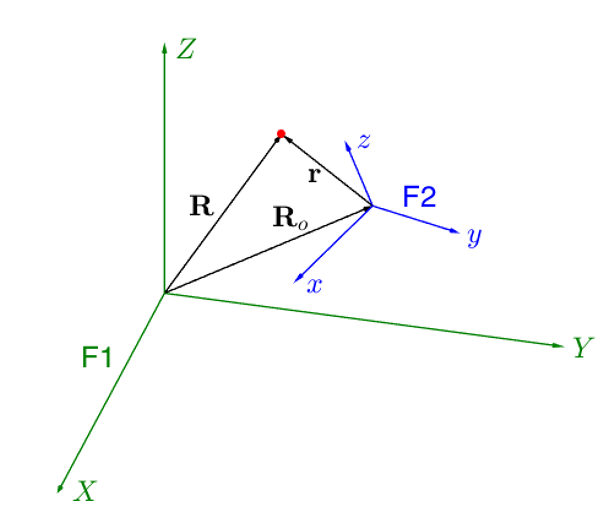
\includegraphics[scale=0.8]{AerospaceApplications/images/RFs.png}
\end{figure}

\noindent
In the above figure the following quantities are shown and a generic particle {\color{red}(in red)} is drawn: 
\begin{equation}
    \begin{aligned}
        &\mathbf{R} = X\mathbf{I} + Y \mathbf{J} + Z \mathbf{K}
        &\text{Position of the particle in F1}\\
        &\mathbf{r} = x \mathbf{i} + y \mathbf{j} + z \mathbf{k}
        &\text{Position of the particle in F2}\\
        &\mathbf{R_O}=X_O \mathbf{I} + Y_O \mathbf{J} + Z_O \mathbf{K}
        &\text{Position in F1 of the O of F2}
    \end{aligned}
\end{equation}
From the geometry follows that $\mathbf{R=R_O+r}$. One wonder at this point \textbf{what is the relation between $X$, $Y$, $Z$ and $x$, $y$, $z$}, using the given former properties we can write:
\begin{equation*}
    \begin{aligned}
        &X = \mathbf{R \cdot I} = \mathbf{(R_O+r) \cdot I} = 
        X_O + x\mathbf{I \cdot i} + y\mathbf{I \cdot j} + 
        z\mathbf{I \cdot k}\\ 
        &Y = \mathbf{R \cdot J} = \mathbf{(R_O+r) \cdot J} = Y_O + x\mathbf{J \cdot i} + y\mathbf{J \cdot j} + 
        z\mathbf{J \cdot k} 
         \\
        &Z = \mathbf{R \cdot K} = \mathbf{(R_O+r) \cdot K} =Z_O + x\mathbf{K \cdot i} + y\mathbf{K \cdot j} + 
        z\mathbf{K \cdot k} \\    
    \end{aligned}
\end{equation*}

Expressed in matrix form:

\begin{equation*}
    \begin{bmatrix}
        X\\Y\\Z
    \end{bmatrix} = 
    \begin{bmatrix}
        X_O\\Y_O\\Z_O
    \end{bmatrix}+
    \begin{bmatrix}
        \mathbf{I \cdot i}&\mathbf{I \cdot j}&\mathbf{I \cdot k}\\
        \mathbf{J \cdot i}&\mathbf{J \cdot j}&\mathbf{J \cdot k}\\
        \mathbf{K \cdot i}&\mathbf{K \cdot j}&\mathbf{K \cdot  k }
    \end{bmatrix}
    \begin{bmatrix}
        x\\y\\z
    \end{bmatrix}, \mathbf{T} \doteq \begin{bmatrix}
        \mathbf{I \cdot i}&\mathbf{I \cdot j}&\mathbf{I \cdot k}\\
        \mathbf{J \cdot i}&\mathbf{J \cdot j}&\mathbf{J \cdot k}\\
        \mathbf{K \cdot i}&\mathbf{K \cdot j}&\mathbf{K \cdot  k }
    \end{bmatrix}
\end{equation*}
The dot products $\mathbf{I \cdot i}$, $\mathbf{I \cdot j}$... represents the \textbf{direction cosine angles} which the axis of one reference frame forms with respect to the other. $\mathbf{T}$ is the \textit{direction cosine matrix}(\textbf{DCM}). 
In literature the DCM can be expressed as:
\begin{equation*}
  \mathbf{T}=\begin{bmatrix}
        T_{11}&T_{12}&T_{13}\\
        T_{21}&T_{22}&T_{23}\\
        T_{31}&T_{32}&T_{33}
    \end{bmatrix}=[T_{ij}]
\end{equation*}
and from the moment that translation and rotation can be studied indipendently, without loss of generality we can assume $\mathbf{R}_O=0$, then the $\mathbf{T}$ becomes a \textbf{transformation matrix} and in particular
\begin{equation*}
    \begin{bmatrix}
        \ X \ \\ \ Y \ \\\ Z \
    \end{bmatrix} = 
    \mathbf{T} 
    \begin{bmatrix}
       \ x \ \\ \ y \ \\ \ z \
    \end{bmatrix}
\end{equation*}
Furthermore, there are \textit{two different interpretation:}
\begin{itemize}
    \itemsep0em
    \item \textbf{Coordinate transformation} from F2 to F1 another term used to indicate this concept is \textit{alias}; 
    \item \textbf{Rotation} of vectors in a given fixed frame, so from F1 to F2, where F2 is the fixed one, another term to indicate this is \textit{alibi}.
\end{itemize}

\subsubsection*{\color{red} Some examples}
Let us consider some examples in 2D, the DCM assumes the form:
\begin{equation*}
    \mathbf{T} = \begin{bmatrix}
        \cos\theta&-\sin\theta\\
        \sin\theta&cos\theta
    \end{bmatrix}
\end{equation*}
From the moment that $z=0$, the third row and the third column of the complete matrix $\mathbf{T}$ disappear.\\

\noindent
{\color{blue} 
\textbf{(\#1) 2D-Coordinate transformation (alias) F2$\to$F1}
}\\
Let us assume that a reference frame F2 is rotated with respect to F1 of an angle $\theta=0.15\pi$, and a particle in F2 is given by
\begin{equation*}
    \mathbf{r} = 0.5\mathbf{i}+0.3\mathbf{j} =
    \begin{bmatrix}
        0.5\\0.3
    \end{bmatrix}
\end{equation*}
The particle coordinates in F1 are obtained through the following transformation
\begin{equation*}
    \begin{bmatrix}
        \ X \ \\ \ Y \
    \end{bmatrix} = \mathbf{Tr} 
\end{equation*}

\begin{figure}[h]
    \centering
    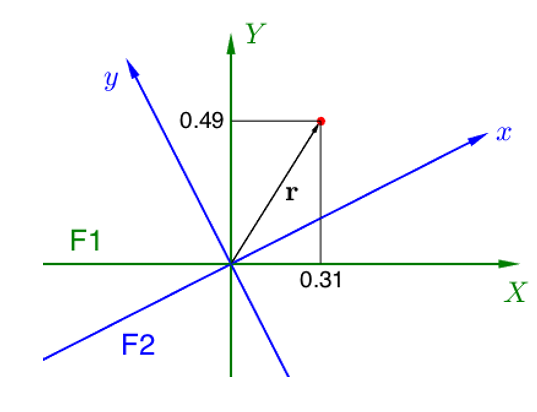
\includegraphics[scale=0.6]{AerospaceApplications/images/coord_transf.png}
    \caption{1st interpretation: Coordinate transformation}
\end{figure}

\noindent
{\color{blue} \textbf{(\#2) 2D-Rotation (alibi) F1$\to$F2}}\\
This time, let us consider a \textbf{vector} $\mathbf{r}$ that in the reference frame F2 is represented by
\begin{equation*}
    \mathbf{r} = \begin{bmatrix}
        \ 0.5 \ \\
        \ 0.3 \
    \end{bmatrix}
\end{equation*}
We can obtain a \textbf{rotated vector} $\mathbf{r}'$ in the same reference frame(fixed) applying the transformation $\mathbf{T}$: 
\begin{equation*}
    \mathbf{r}'=\mathbf{T}\cdot\mathbf{r}
\end{equation*}

\begin{figure}[h]
    \centering
    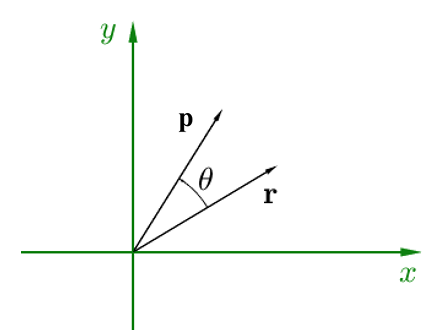
\includegraphics[scale=1]{AerospaceApplications/images/rotation_transf.png}
    \caption{2nd interpretation: rotation in a fixed frame}
\end{figure}

\noindent
{\color{blue} \textbf{(\#3) Rotation of a square in 2D}}
The concept of rotation can be generalized to a 2D-figure like a square for example. A square in 2D can be represented by a matrix $\mathbf{S}\in\mathbb{R}^{2,4}$, which contains by column the (2D)coordinates of the vertices.\\
If we want rotate a square of an angle $\theta$ we can apply the DCM (computed in the angle $\theta$) obtaining a \textbf{rotated square} $\mathbf{S'}$ as follows:
\begin{equation*}
    \mathbf{S'} = \mathbf{T} \cdot \mathbf{S}
\end{equation*}

\begin{figure}[h]
    \centering
    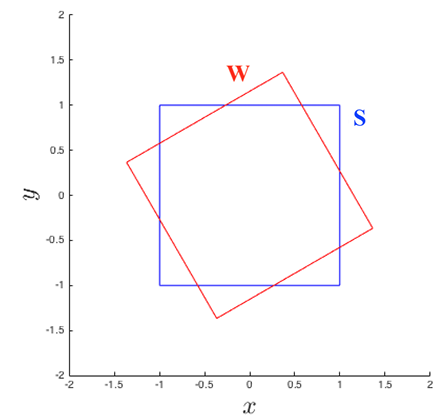
\includegraphics[scale=1]{AerospaceApplications/images/square_rot.png}
    \caption{Rotation of a square}
\end{figure}

\subsection{Euler angles}
In \textbf{three dimensions} we define the \textit{elementary rotation matrices}
\begin{equation*}
    \begin{aligned}
        &\mathbf{T}_1(\phi) = 
        \begin{bmatrix}
            1&0&0\\
            0&\cos\phi&-\sin\phi\\
            0&\sin\phi&cos\phi
        \end{bmatrix} & \text{Rotation about $X$ (or x) of $\phi$ }\\
        &\mathbf{T}_2(\theta) = 
        \begin{bmatrix}
            \cos\theta&0&\sin\theta\\
            0&1&0\\
            -\sin\theta&0&\cos\theta
        \end{bmatrix}  & \text{Rotation about $Y$ (or y) of $\theta$ } \\
        &\mathbf{T}_3(\psi) = \begin{bmatrix}
            \cos\psi&-\sin\psi&0\\
            sin\psi&cos\psi&0\\
            0&0&1
        \end{bmatrix}
        & \text{Rotation about $Z$ (or z) of $\psi$ }\\
    \end{aligned}
\end{equation*}
The interesting thing is that \textbf{any rotation in 3D} can be expressed as a product of $\mathbf{T}_1$, $\mathbf{T}_2$, $\mathbf{T}_3$, moreover the three angles $\phi, \theta, \psi$ are the so-called \textbf{Euler angles}.\\
There are 12 possible combinations of the three elementary matrices of rotations (with non sequentially repeated indexes) they can be divided in \textbf{two groups}: 
\begin{itemize}
    \itemsep0em
    \item[\ding{70}] \textbf{6 Tait-Bryan rotations} the most used are 123 and 321
    \item[\ding{70}] \textbf{6 proper Euler rotations} the most common is 313
\end{itemize}

As they are very used their expression is reported below:

{\color{red}\subsubsection{Tait-Bryan $\mathbf{T}_{123}$}}
\begin{equation*}
    {\large{
        \mathbf{T}_{123}=\begin{bmatrix}
            \cos\theta \cos \psi &
            -cos\theta \sin \psi &
            \sin\theta \\
            \cos\phi\sin\psi + \sin\phi\sin\theta\cos\psi&
            \cos\phi\cos\psi - \sin\phi\sin\theta\sin\psi&
            -\sin\phi\cos\theta\\
            \sin\phi\sin\psi-\cos\phi\sin\theta\cos\psi &
            \sin\phi\cos\psi+\cos\phi\sin\theta\sin\psi &
            \cos\phi\cos\theta
        \end{bmatrix}
    }}
\end{equation*}

{\color{red}\subsubsection{Tait-Bryan $\mathbf{T}_{321}$}}
\begin{equation*}
    {\large{
        \mathbf{T}_{321} = \begin{bmatrix}
            \cos\theta \cos\psi & -\cos\phi \sin\psi +\sin\phi\sin\theta\cos\psi & \sin\phi\sin\psi +\cos\phi \sin\theta \cos\psi\\
            \cos\theta \sin\psi & \cos\phi \cos\psi +\sin\phi\sin\theta\sin\psi & -\sin\phi\cos\psi +\cos\phi \sin\theta \sin\psi\\
            -\sin\theta & \sin\phi\cos\theta&\cos\phi\cos\theta
        \end{bmatrix}
    }}
\end{equation*}


{\color{red}\subsubsection{Proper Euler $\mathbf{T}_{313}$}}
\begin{equation*}
    {\large{
        \mathbf{T}_{313} = \begin{bmatrix}
            \cos\phi \cos\psi - \sin\phi \cos\theta \sin\psi & -\cos\phi \sin\psi -\sin\phi \cos\theta \cos\psi & \sin\phi \sin\theta\\
            \sin\phi \cos\psi + \cos\phi \cos\theta \sin\psi & -sin\phi \sin\psi + \cos\phi \cos\theta \cos\psi & -cos\phi \sin\theta\\
            \sin\theta \sin\psi & \sin\theta \cos\psi & \cos\theta 
    \end{bmatrix}
    }} 
\end{equation*}

\subsection{Rotation matrices general properties}
The following are \textbf{general properties} related to the rotation matrices. \textbf{Notation}: we indicate with $\mathbf{T}_{\diamond}$ any composition of the elementary rotation matrices (with non-sequentially repeated elements).\\
Matrices $\mathbf{T}_{\diamond}$ have the following properties:
\begin{itemize}
    \itemsep0em
    \item[\ding{70}] They are \textbf{linear transformations}, from the product of linear matrices;
    \item[\ding{70}] They are \textbf{orthogonal matrices}, that is matrices whose columns are composed of real entries and are \textbf{orthonormal}. The most important property is: 
    $$\mathbf{T}_{\diamond}^T=\mathbf{T}_{\diamond}^{-1}, \quad 
    \mathbf{T}_{\diamond}^{T}\mathbf{T}_{\diamond}=\mathbf{T}_{\diamond}\mathbf{T}_{\diamond}^T=\mathbf{I}$$
    \textbf{orthogonal transformations} preserve:
    \begin{itemize}
        \itemsep0em
        \item the \textbf{length} of the vectors;
        \item the \textbf{angles} between the vectors;
    \end{itemize}
    $$\text{length} + \text{angles} \Longrightarrow \textbf{shape preserved}$$
    \item[\ding{70}] Their \textbf{eigenvalues} are always $\{1, \pm e^{j\beta}\}$, their \textbf{determinant} always equal to 1;
\end{itemize} 

{\color{blue}\subsubsection{Singularities, Gimbal lock}}
For certain values of $\theta$ some matrices can present some \textbf{singularities}, for example the matrix $\mathbf{T}_{123}$. For example if $\theta=\frac{\pi}{2}$ only the sum $(\psi+\phi)$ can be determined and this results in a \textbf{loss of degree of freedom} $\Longrightarrow$ this phenomenon is also known as \textbf{gimbal lock} and affect all the \textit{gyroscopes} in which two out of three axes are aligned and this results in a loss of a degree of freedom, in \textit{normal situations} the three axis, instead, can rotate indipendently.
In order to overcome this problem, we use non minimal representation in which instead of only three variables, are used \textbf{four variables}.\\
More in general, \textbf{there is always a gimbal lock} when: 
\begin{itemize}
    \itemsep0em
    \item[\ding{70}] In the \textbf{Tait-Bryan rotations}, $\cos\theta=0$;
    \item[\ding{70}] In the \textbf{Proper Euler rotations}, when occurs that $\sin\theta=0$   
\end{itemize}
This singularities cause problems in the \textit{kinematic equation} like divergent behaviour, this is the reason why alternative method to manage these situations are required.

\begin{figure}[h]  
    \centering
    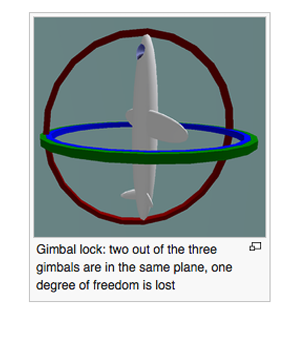
\includegraphics[scale=1.3]{AerospaceApplications/images/gimbal_lock.png}
    \caption{Gimbal lock example}
\end{figure}

\subsection{Euler's rotation theorem}
The following theorem is very important because it introduces an alternative way to describe rotations: \\

\hspace*{-5mm}
\begin{tikzpicture}
\node [mybox] (box){%
    \begin{minipage}{.96\textwidth}     %Larghezza del box
        \large{
            \textbf{\underline{Theorem (angle-axis representation)}}
            \begin{itemize}
                \itemsep0em
                \item[(i)] Any rotation of a rigid body where a point is fixed is \textbf{equivalent} to a rotation in which the rotation axis passes through the fixed point; 
                \item[(ii)] The rotation axis is the \textbf{eigenvector} $\mathbf{u}$ corresponding to the eigenvalues 1 of the rotation matrix. 
                \vspace{0.2cm}
            \end{itemize} 
        }
    \end{minipage}
};
\end{tikzpicture}%

\vspace{0.5cm}
\noindent
\textbf{\textit{Proof}}\\
The rotation matrix $\mathbf{T}_{\diamond}$ has a unitary eigenvalue, it holds (from the definition) that: $\mathbf{T}_{\diamond}\mathbf{u}=\mathbf{u}$, so the rotation does not change the direction $\mathbf{u}$, which is the rotation axis. $_\square$\\

From this theorem, follows that \textit{any rotation} can be described by using two quantities involving four variables: 
\begin{itemize}
    \itemsep0em
    \item[\ding{70}] An angle $\beta$ (1 variable)
    \item[\ding{70}] A rotation axis $\mathbf{u}$ (3 variables)
\end{itemize}
{
\huge{
\begin{equation*}
    \mathbf{T} \equiv \mathbf{T}(\beta, \mathbf{u})
\end{equation*}}
}

\subsection{Quaternions}
\textbf{Quaternions} are mathematical object introduced by Hamilton. They are: (i) an extension of the concept of \textit{Complex numbers}, (ii) are useful and more robust tool to describe \textbf{rotations}. \\
\textbf{Complex numbers} are element of a 2D-vector space whose basis is $\{1,\mathbf{i}\}$. Each element can be expressed as a linear combination of these two elements.\\
In an equivalent way we can state that:\\

\hspace*{-5mm}
\begin{tikzpicture}
\node [mybox] (box){%
    \begin{minipage}{.96\textwidth}     %Larghezza del box
        {
            \large{
                \textbf{DEFINITION (QUATERNIONS)}\\
                The quaternions are element of a 4D-dimensional vector space whose basis is $\{1, \mathbf{i, j, k}\}$, where is defined a particular \textbf{product} indicated with $\otimes$. The following properties hold:
                \begin{equation*}
                    \begin{aligned}
                        &\mathbf{i}^2=\mathbf{j}^2=\mathbf{k}^2=\mathbf{i\otimes j \otimes k}=-1\\
                        &\mathbf{i}\otimes\mathbf{j}=-\mathbf{j}\otimes\mathbf{i}=\mathbf{k}\\
                        &\mathbf{j}\otimes\mathbf{k}=-\mathbf{k}\otimes\mathbf{j}=\mathbf{i}\\
                        &\mathbf{k}\otimes\mathbf{i}=-\mathbf{i}\otimes\mathbf{k}=\mathbf{j}
                    \end{aligned}
                \end{equation*}
            }
        }
    \end{minipage}
};
\end{tikzpicture}%

\noindent
As we introduced a new mathematical object we have to define a set of properties and some notation.

{\color{red} \subsubsection*{Notation}}

One can indicate a quaternion using one of the following notations:
{\large{
    \begin{align*}
        \mathfrak{q} \quad &= \quad q_0+q_1\mathbf{i}+q_1\mathbf{j}+q_2\mathbf{k}=\\
                     &= \quad q_0+\mathbf{q}=\\
                     &=\quad (q_0, q_1, q_2, q_3)=\\
                     &=\quad  (q_0, \mathbf{q})=\begin{bmatrix}
                        \ q_0 \ \\\ \mathbf{q} \
                     \end{bmatrix}
    \end{align*}
}}

\begin{itemize}
    \itemsep0em
    \item $q_0$ is the \textit{real part}
    \item $\mathbf{q}$ is the so-called \textit{vector part}
    \item if $q_0=0$, the resulting quaternion $\mathfrak{q}=(0,\mathbf{q})$ is said to be \textit{pure}
\end{itemize}

{\color{red} \subsubsection*{Null element}}
\noindent
The \textbf{null element} of the quaternion vector space is
{\Large{
    \begin{equation*}
        \mathfrak{O} = (0, \mathbf{0})
    \end{equation*}
}
}

{\color{red} \subsubsection*{Complex conjugate}}
\noindent
The \textbf{complex conjugate} $\mathfrak{q}^*$ of a quaternion $\mathfrak{q}=q_0+\mathbf{q}$ is
{\Large{
    \begin{align*}
        \mathfrak{q}^*=q_0-q=\begin{bmatrix}
            q_0\\-\mathbf{q}
        \end{bmatrix}=(q_0, -\mathbf{q})
    \end{align*}
}} 

{\color{red} \subsubsection*{Norm}}
\noindent
We simply define the \textbf{quaternion norm} as
{\Large{
    \begin{equation*}
        \vert \mathfrak{q} \vert = \Vert \mathfrak{q} \Vert = \vert \mathfrak{q}^* \vert=\sqrt(q \cdots q^* )=
        \sum_{i=0}^3 {q_i}^2
    \end{equation*}
}}

{\color{red} \subsubsection*{Reciprocal element}}
\noindent
Given a quaternion $\mathfrak{q}$, the reciprocal element $\mathfrak{q}^-1$ is
{\Large{
    \begin{equation*}
        \mathfrak{q}^{-1}=\frac{\mathfrak{q}^*}{\Vert \mathfrak{q} \Vert}
    \end{equation*}
}} 

{\color{red} \subsubsection*{Sum}}
\noindent
The \textbf{sum} of two quaternions $\mathfrak{q}$ and  $\mathfrak{p}$ is
{\Large{
    \begin{equation*}
        \mathfrak{q}+\mathfrak{p}=q_0+p_0+\mathbf{q}+\mathbf{p}
    \end{equation*}
}}

{\color{red} \subsubsection*{Dot product}}
\noindent
The \textbf{dot product} of two quaternions $\mathfrak{q}$ and $\mathfrak{p}$ is
{\Large{
    \begin{equation*}
        \mathfrak{q} \cdot \mathfrak{p} = 
        \sum_{i=0}^3 {q_i p_i}
    \end{equation*}
}}
 
{\color{red} \subsubsection*{Quaternion product (Hamilton product)}}
\noindent
Given two quaternions $\mathfrak{q} \ \text{and} \ \mathfrak{p}$ we define the \textbf{Hamilton product} as:
{\Large{
    \begin{align*}
        \mathfrak{q} \otimes \mathfrak{p} &= 
        (q_0+\mathbf{q}) \otimes (p_0+\mathbf{p}) = (...)\\
        &= (q_0p_0-\mathbf{q}\cdot\mathbf{p})+(q_0\mathbf{p}+p_0\mathbf{q}+\mathbf{q}\times\mathbf{p})
    \end{align*}
}}
Where $\mathbf{q}\times\mathbf{p}$ is the cross product
\begin{equation*}
    \mathbf{q}\times\mathbf{p}=
    \begin{bmatrix}
        \ q_2p_3-q_3p_2 \ \\
        \ q_3p_1-q_1p_3 \ \\
        \ q_1p_2-q_2p_1 \
    \end{bmatrix}
\end{equation*}
Also the quaternion vector space has an \textbf{identity element} equal to
{\Large{
    \begin{equation*}
        \mathfrak{I} = (1, \mathbf{0})
    \end{equation*}
}}

\subsection{Describe rotations through quaternions}
Through this subsection we will entry into details of why quaternions can be useful to describe rotations. At first, we have to say that given a vector $\mathbf{r}$ with component $x,y, z$, its 4D extension is $(0, \mathbf{r})$. We have seen thanks to the \textbf{angle-axis} representation that a rotation of the vector $\mathbf{r}$ of an angle $\beta$ and rotation axis $\mathbf{u}$ is $\mathbf{p}=\mathbf{T}(\beta, \mathbf{u})\mathbf{r}$. \\
For given $\beta$ and $\mathbf{u}$, the associated unit quaternion is defined as
{\large{
    \begin{equation*}
        \mathfrak{q} \doteq 
        \bigg( 
            \cos\frac{\beta}{2}, \
            \mathbf{u} \sin\frac{\beta}{2} \
        \bigg)=
        \bigg( 
            \cos\frac{\beta}{2}, \
            u_1 \sin\frac{\beta}{2}, \
            u_2 \sin\frac{\beta}{2},\
            u_3 \sin\frac{\beta}{2} \
        \bigg)
    \end{equation*}
}}
\noindent
The \textit{components} of this vector are called \textbf{Euler parameters}.\\

\hspace*{-5mm}
\begin{tikzpicture}
\node [mybox] (box){%
    \begin{minipage}{.96\textwidth}     %Larghezza del box
        \Large{
            \textbf{Theorem}
            The \textit{rotated vector} $\mathbf{p}$ can be defined as 
            \begin{equation*}
                (0,\mathbf{p}) = \mathfrak{q} \otimes (0, \mathbf{r}) \otimes \mathfrak{q}^*
            \end{equation*}
        }
    \end{minipage}
};
\end{tikzpicture}%

\noindent
From the moment that we can associate each \textit{angle-axis} representation to a specific quaternion, we can retrieve the quaternions of the \textit{elementary rotation matrices} as follows:
{\Large{
    \begin{align*}
        &\mathbf{T}_1(\phi) \longleftrightarrow
        \mathfrak{q}_1 = \bigg(\cos \frac{\phi}{2}, \sin \frac{\phi}{2}, 0, 0 \bigg)\\
        &\mathbf{T}_2(\theta) \longleftrightarrow 
        \mathfrak{q}_2=\bigg(\cos \frac{\theta}{2}, 0, \sin \frac{\theta}{2}, 0 \bigg)\\
        &\mathbf{T}_3(\psi) \longleftrightarrow 
        \mathfrak{q}_3=\bigg(\cos \frac{\psi}{2}, 0, 0, \sin\frac{\psi}{2} \bigg)
    \end{align*}
}}
At this point we can note that any rotation can be expressed in the form an Hamilton product between the \textbf{quaternions}, that is 
{\Large{
    \begin{equation*}
        \mathfrak{q} = 
        \mathfrak{q}_1 \otimes
        \mathfrak{q}_2 \otimes
        \dots \otimes
        \mathfrak{q}_n
    \end{equation*}
}}
The \textbf{inverse rotation} is
{\Large{
    \begin{equation*}
        \mathfrak{q}^{-1} = \mathfrak{q}^*
    \end{equation*}
}}

\section{Attitude kinematics}
The objective of this paragraph is to derive the \textbf{kinematic equations} for a generic \textit{rigid body} in rotational motion, these equations are crucially important for the \textbf{spacecraft attitude control}.\\
In general, the dynamic and kinematic equations can be seen as a \textbf{series of two nonlinear systems}.

\begin{figure}[h]
    \centering 
    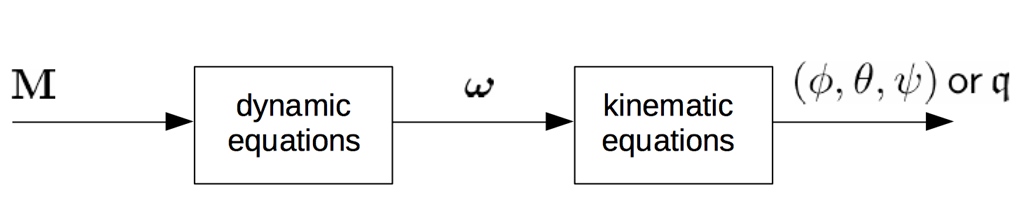
\includegraphics[scale=0.7]{AerospaceApplications/images/kin_dyn_series.png}
\end{figure}

In this figure:
\begin{itemize}
    \itemsep0em
    \item The \textbf{dynamic equations} block has got as input an external torque $\mathbf{M}$ and as output the angular velocity vector $\boldsymbol{\omega}$.
    \item The \textbf{kinematic equations} block has got as input the output of dynamic block, then the angular velocity  $\boldsymbol{\omega}$, as output one between the \textbf{Euler angles} $(\phi, \theta, \psi)$ and the rotation \textbf{quaternion} $\mathfrak{q}$.
\end{itemize}

Then, the overall system has: input $\mathbf{M}(t)$ and ouput $(\phi, \theta, \psi)$ or $\mathfrak{q}$ which represents the output to control. For instance the rotation is crucial in order to obtain a certain orientation of the spacecraft toward a certain direction. 

The classical setting in this case is considering that the rigid body is rotating with respect to some \textbf{observer reference frame} \textsf{OF}, with an \textit{angular velocity} $\boldsymbol{\omega}=\omega_1\mathbf{b}_1 + \omega_2\mathbf{b}_2+\omega_3\mathbf{b}_3$ in which:
\begin{itemize}
    \itemsep0em
    \item $\omega=\vert \boldsymbol{\omega} \vert$ is the speed of rotation; 
    \item The unit vector $\frac{\boldsymbol{\omega}}{\vert \boldsymbol{\omega} \vert}$ is the \textit{rotation axis}.
\end{itemize}

We can individuate two \textit{reference frames}: the \textbf{observer frame} (\textsf{OF}) and the \textbf{body frame} (\textsf{BF}), when we introduce some reference frames we must give some information like: where is the origin? Which are the unit vectors? And the axis? In our case we have:
\begin{enumerate}
    \item \textbf{Observer frame}(\textsf{OF}) $\begin{cases}
        \text{origin: somewhere}\\
        \text{unit vectors}: \{\mathbf{i}_1 
        \mathbf{i}_2, \mathbf{i}_3\}\\
        \text{axis:} X, Y, Z 
    \end{cases}$
    \item \textbf{Body frame}(\textsf{BF}) $\begin{cases}
        \text{origin: CoM of Rigid body }\to \text{rotates with the body}\\
        \text{unit vectors: } \{\mathbf{b}_1, \mathbf{b}_2, \mathbf{b}_3\}\\
        \text{axis}: x, y, z
    \end{cases}$
\end{enumerate} 

\begin{figure}[h]
    \centering
    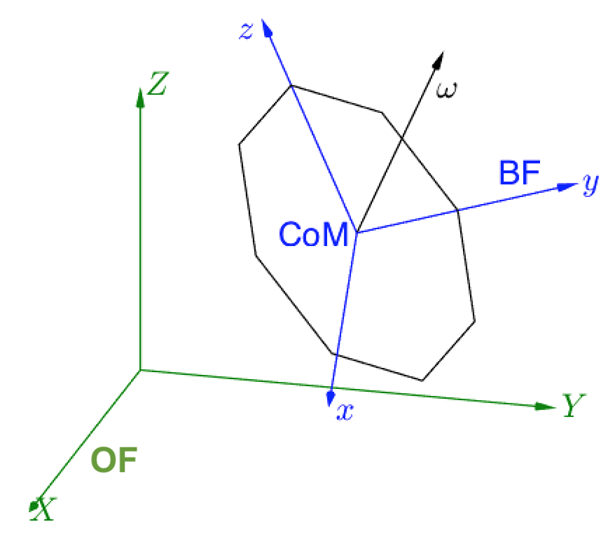
\includegraphics[scale=0.7]{AerospaceApplications/images/OF_BF.png}
    \caption{ \textsf{Observer and Body frames for a generic rigid body}} 
\end{figure}

From the moment that the rotation from \textsf{OF} to \textsf{BF} can be described by using either the Euler angles or the quaternions, we can derive some kinematic equations for both type of representation. Before doing this, it is important to give the definition of what is the \textbf{derivative of a vector}.

\subsection{Vector derivative}
Any physical vector can be expressed in the form
{\large{
    \begin{equation}
        \mathbf{r} = x \mathbf{b}_1 +
                     y \mathbf{b}_2 +
                     z \mathbf{b}_3
    \end{equation}
}}
If one makes the \textbf{derivative} of such vector applying the basic rules from the differential calcus, it will be obtained
{\large{
    \begin{align}
        \dot{\mathbf{r}} = \dot{x} \mathbf{b}_1 +
                           \dot{y} \mathbf{b}_2 +
                           \dot{z} \mathbf{b}_3 +
                           x \dot{\mathbf{b}}_1 +
                           y \dot{\mathbf{b}}_2 + 
                           z \dot{\mathbf{b}}_3
    \end{align}
}}
Between two different time instants, the difference vector is
\begin{equation}
    \delta{\mathbf{b}}_i = \delta\boldsymbol{\theta} \times \mathbf{b}_i 
\end{equation}
but if the vector $\mathbf{r}$ is rotating with an angular velocity $\boldsymbol{\omega}$, then the angle $\delta\boldsymbol{\theta}$ is equal to $\delta\mathbf{\theta} \doteq \boldsymbol{\omega}\delta t$. When $\delta t\to 0$, the vectors before and after the infinitesimal rotation are very similar, then the vector $\delta\mathbf{b}_i$ becomes $\delta\mathbf{b}_i=\boldsymbol{\omega}\times \mathbf{b}_i$. Putting all together we have:
{\large{
    \begin{equation}
        \dot{\mathbf{r}} = \dot{\mathbf{r}}_B + \boldsymbol{\omega} \times \mathbf{r}
    \end{equation}
}}
Where $\dot{\mathbf{r}}_B=\dot{x} \mathbf{b}_1 +
\dot{y} \mathbf{b}_2 +
\dot{z} \mathbf{b}_3$ is the derivative of $\mathbf{r}$ in the \textbf{body frame}, while $\dot{\mathbf{r}}$ is the derivative of $\mathbf{r}$ in the \textbf{observer frame}.

\subsection{Euler angles kinematic}
We want to retrieve a relation between the input $\mathbf{\omega}(t)$ and the \textbf{Euler angles} $(\phi, \theta, \psi)$. Unfortunately, for the rotations it is not so easy as in the case of \textit{traslational motion}, moreover the relation between the Euler angles derivatives and the components of the angular velocity is NOT the identity matrix. We will provide the kinematic equations for the most used \textit{Tait-Bryan} rotations and for the \textit{Proper Euler angle} rotation. [The derivation of such formulas is not trivial at all].\\
It is interesting to note that, in the case we use this type of representation we have some \textbf{singularities} in the equations due to the \textit{gimbal-lock} phenomenon. On the other hand, by using a non-minimal representation, rotations described through the quaternions is free from this problem.

\subsubsection{Tait-Bryan 321}
It can be demonstrated that
\begin{equation}
        \begin{bmatrix}
            \omega_1\\
            \omega_2\\
            \omega_3
        \end{bmatrix} = 
        \begin{bmatrix}
            1&0&-\sin\theta\\
            0&\cos\phi&\sin\phi\cos\theta\\
            0&-\sin\theta&\cos\phi\cos\theta
        \end{bmatrix}
        \begin{bmatrix}
            \dot{\phi}\\
            \dot{\theta}\\
            \dot{\psi}
        \end{bmatrix}
\end{equation}
We can invert the matrix and we can obtain the \textit{Tait-Bryan 321 kinematic equation}:
\begin{equation}
    \begin{bmatrix}
        \dot{\phi}\\
        \dot{\theta}\\
        \dot{\psi}
    \end{bmatrix}=\frac{1}{\cos\theta}\begin{bmatrix}
        \cos\theta&\sin\phi\sin\theta&\cos\phi\sin\theta\\
        0&\cos\phi\cos\theta&-\sin\phi\cos\theta\\
        0&\sin\phi&\cos\phi
    \end{bmatrix}\begin{bmatrix}
        \omega_1\\
        \omega_2\\
        \omega_3
    \end{bmatrix}
\end{equation}
When $\cos\theta=0$ the gimbal-lock occurs, then we have a singularity in the kinematic equations.

\subsubsection{Tait-Bryan 123}
It can be demonstrated that
\begin{equation}
        \begin{bmatrix}
            \omega_1\\
            \omega_2\\
            \omega_3
        \end{bmatrix} = 
        \begin{bmatrix}
           \cos\theta\cos\psi&\sin\psi&0\\
           -\cos\theta\sin\psi&\cos\psi&0\\
           \sin\theta&0&1
        \end{bmatrix}
        \begin{bmatrix}
            \dot{\phi}\\
            \dot{\theta}\\
            \dot{\psi}
        \end{bmatrix}
\end{equation}
We can invert the matrix and we can obtain the \textit{Tait-Bryan 123 kinematic equation}:
\begin{equation}
    \begin{bmatrix}
        \dot{\phi}\\
        \dot{\theta}\\
        \dot{\psi}
    \end{bmatrix}=\frac{1}{\cos\theta}\begin{bmatrix}
        \cos\psi&-\sin\psi&0\\
        \cos\theta\sin\psi&\cos\theta\cos\psi&0\\
        -\sin\theta\cos\psi&\sin\theta\sin\psi&\cos\theta
    \end{bmatrix}\begin{bmatrix}
        \omega_1\\
        \omega_2\\
        \omega_3
    \end{bmatrix}
\end{equation}
When $\cos\theta=0$ the gimbal-lock occurs, then we have a singularity in the kinematic equations.



\subsubsection{Proper-Euler 313}
It can be demonstrated that
\begin{equation}
        \begin{bmatrix}
            \omega_1\\
            \omega_2\\
            \omega_3
        \end{bmatrix} = 
        \begin{bmatrix}
           \sin\theta\sin\psi&\cos\psi&0\\
           \sin\theta\cos\psi&-\sin\psi&0\\
           \cos\theta&0&1
        \end{bmatrix}
        \begin{bmatrix}
            \dot{\phi}\\
            \dot{\theta}\\
            \dot{\psi}
        \end{bmatrix}
\end{equation}
We can invert the matrix and we can obtain the \textit{Tait-Bryan 313 kinematic equation}:
\begin{equation}
    \begin{bmatrix}
        \dot{\phi}\\
        \dot{\theta}\\
        \dot{\psi}
    \end{bmatrix}=\frac{1}{\sin\theta}\begin{bmatrix}
        \sin\psi&\cos\psi&0\\
        \sin\theta\cos\psi&-\sin\theta\sin\psi&0\\
        \cos\theta\sin\psi&-\cos\theta\cos\psi&\sin\theta
    \end{bmatrix}\begin{bmatrix}
        \omega_1\\
        \omega_2\\
        \omega_3
    \end{bmatrix}
\end{equation}
When $\cos\theta=0$ the gimbal-lock occurs, then we have a singularity in the kinematic equations.

\subsection{Quaternion kinematic}
The \textbf{quaternion kinematic} can be written in different equivalent forms:
\begin{align}
    &\dot{\mathfrak{q}}=\frac{1}{2}\mathfrak{q}\otimes(0,\boldsymbol{\omega})\\
    &\dot{\mathfrak(q)}=\frac{1}{2}\boldsymbol{\Omega}q\\
    &\dot{\mathfrak{q}}=\frac{1}{2}\mathbf{Q}\boldsymbol{\omega}
\end{align}
where the matrices $\boldsymbol{\Omega}$ and $\mathbf{Q}$ are defined as follows
\begin{equation*}
    \boldsymbol{\Omega}\doteq\begin{bmatrix}
        0&-\omega_1&-\omega_2&-\omega_3\\
        \omega_1&0&\omega_3&-\omega_2\\
        \omega_2&-\omega_3&0&\omega_1\\
        \omega_3&\omega_2&-\omega_1&0
    \end{bmatrix}, \quad 
    \mathbf{Q}\doteq \begin{bmatrix}
        -q_1&-q_2&-q3\\
        q_0&-q_3&q_2\\
        q_3&q_0&-q_1\\
        -q_2&q_1&q_0
    \end{bmatrix}
\end{equation*} 

\subsection{Discussion}
Through these paragraphs we have found the \textbf{kinematic equations} in the general form
{\large{
    \begin{equation}
        \dot{\mathbf{x}} = A(\mathbf{x})\boldsymbol{\omega}
    \end{equation}
}}
where $\mathbf{x}=(\phi, \theta, \psi)$ or $\mathbf{x}=\mathfrak{q}$. This is a \textbf{state equation}, with state $\mathbf{x}$ and input $\boldsymbol{\omega}$. State equations allow us to predict the time evolution of a system given a certain initial condition $x_0$ and a given input $\boldsymbol{\omega}(t)$. The solution can be found sometimes analitically, otherwise numerical methods have to be exploited, but in this case a solution - even if approximately - can be always provided.

\section{Attitude dynamics}
In the previous chapter we analysed the equations for the kinematic part of rotations. In this chapter, instead we want to describe the \textbf{attitude dynamic equations} how mentioned they play a fundamental role for the atttitude control of spacecrafts.\\
We use the same setting with two reference frames, the inertial frame (constant $v_O$) and the body frame, a generic particle $m_i$ of the rigid body has got the following properties:

\begin{figure*}[h]
    \centering 
    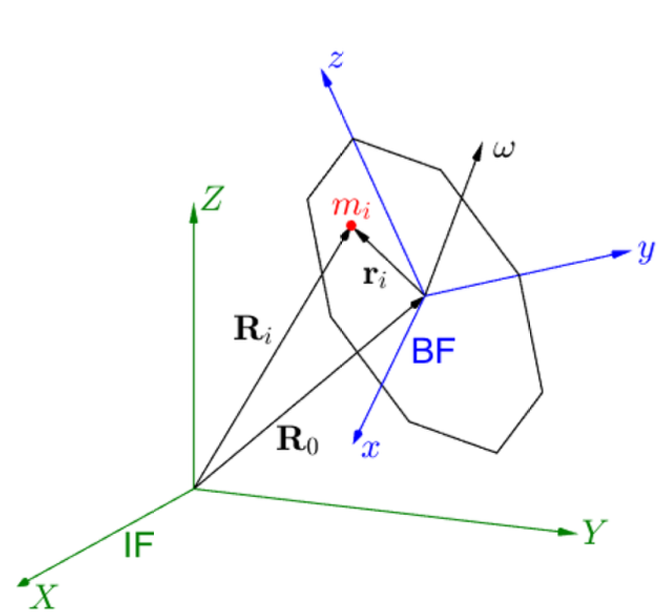
\includegraphics[scale=0.5]{AerospaceApplications/images/IF_BF.png}    
\end{figure*}

\begin{align*}
    &\mathbf{R}_i = X\mathbf{i}_1 +  Y \mathbf{i}_2 + Z \mathbf{i}_3 = \mathbf{R}_O+\mathbf{r}_i\\
    &R_O= X_O\mathbf{i}_1 +  Y_O \mathbf{i}_2 + Z_O \mathbf{i}_3\\
    &\dot{\mathbf{R}}_i = \dot{\mathbf{R}}_O + 
    \dot{\mathbf{r}}_{iB}+\boldsymbol{\omega}\times\mathbf{r}_i\\
    &\mathbf{r}_i=x\mathbf{b}_1+y\mathbf{b}_2+z\mathbf{b}_3\\
    &\mathbf{r}_{iB}=\dot{x}\mathbf{b}_1+\dot{y}\mathbf{b}_2+\dot{z}\mathbf{b}_3\\
    &\boldsymbol{\omega} = \omega_1\mathbf{b}_1+\omega_2\mathbf{b}_2+\omega_3{\mathbf{b}}_3
\end{align*}

\subsection{Angular momentum}
Let us start introducing what is the \textbf{angular momentum} of a particle $m_i$. It is defined as 
\begin{equation}
    \mathbf{H}_i=r_i\times m\dot{\mathbf{R}}_i=
    \mathbf{r}_i \times m_i \big( 
        \dot{\mathbf{R}}_O + 
        \dot{\mathbf{r}}_{iB}+\boldsymbol{\omega}\times\mathbf{r}_i
    \big)
\end{equation}
Being a rigid body the position of the single particle $m_i$ does not change in time, so the term $\mathbf{r}_{iB}=0$, then it will be obtained
\begin{align*}
    \mathbf{H}_i \quad &= \quad \mathbf{r}_i \times m_i 
        \bigg( \dot{\mathbf{R}}_O +\boldsymbol{\omega}\times\mathbf{r}_i\bigg)\\
        &= \quad -\dot{\mathbf{R}}_O\times m_i\mathbf{r}_i+\mathbf{r}_i\times m_i(\boldsymbol{\omega}\times\mathbf{r}_i)
\end{align*}
If we extend the reasing for all the particles of the body we will obtain:
\begin{align*}
    \mathbf{H} \quad &= \quad 
    -\sum_i \dot{\mathbf{R}}_O\times m_i\mathbf{r}_i+
    \sum_i\mathbf{r}_i\times m_i(\boldsymbol{\omega}\times\mathbf{r}_i)\\
    &=\quad -\dot{\mathbf{R}}_O\times \sum_i  m_i\mathbf{r}_i+
    \sum_i\mathbf{r}_i\times m_i(\boldsymbol{\omega}\times\mathbf{r}_i)\\
    &=\quad \sum_i\mathbf{r}_i\times m_i(\boldsymbol{\omega}\times\mathbf{r}_i)
\end{align*}
in which the term $\sum_i  m_i\mathbf{r}_i=\mathbf{0}$ by definition of Center of Mass (CoM). In a rigid body the particle are not discrete, the particles for which we can compute the angular momentum are \textit{infinitesimal}: $m_i\to dm$. We have substancially replace the summation with the integral obtaining at the end:
\begin{equation}
    \mathbf{H} = \int_B{\mathbf{r}\times (\boldsymbol{\omega}\times\mathbf{r})} \ dm
\end{equation}

\subsection{Inertia matrix (o tensor)}
If we perform the products, we will obtain in body coordinates:
\begin{equation}
    \mathbf{H}=\begin{bmatrix}
        J_{11}&J_{12}&J_{13}\\
        J_{21}&J_{22}&J_{23}\\
        J_{31}&J_{32}&J_{33}
    \end{bmatrix}\begin{bmatrix}
        \omega_1\\\omega_2\\\omega_3
    \end{bmatrix}=\boldsymbol{J\omega}
\end{equation}
The matrix $\mathbf{J}$ is the \textbf{inertia matrix} or \textbf{inertia tensor} and it depends only on the properties of the body. The elements $J_{ij}$ are defined as follows:
\begin{align*}
    &\textsf{moments of inertia} \ \begin{cases}
        J_{11}=\int_B (z^2+y^2) \ dm\\
        J_{22}=\int_B (x^2+z^2) \ dm\\
        J_{33}=\int_B (x^2+y^2) \ dm
    \end{cases}\\
    &\textsf{products of inertia} \ \begin{cases}
        J_{12}=J_{21}=-\int_B xy \ dm\\
        J_{13}=J_{31}=-\int_B xz \ dm\\
        J_{23}=J_{32}=-\int_B yx \ dm
    \end{cases}
\end{align*}
The inertia matrix $\mathbf{J}_o$ has real entries and it is symmetric, for the spectral theorem, a \textbf{diagonal matrix} $\mathbf{J}$ such that 
$$\mathbf{J} = \mathbf{T}^T\mathbf{J}_o\mathbf{T}$$
$J=\text{diag}(J_1, J_2, J_3)$ is a diagonal matrix whose entries are the eigenvalues of the non-symmetric matrix $\mathbf{J}_o$.
The matrix $\mathbf{T}=[\mathbf{e}_1 \ \mathbf{e}_2 \ \mathbf{e}_3]$ is a rotation matrix and its columns are the eigenvector of $\mathbf{J}_o$.
At this point we call:
\begin{itemize}
    \item \textbf{Principal moments of inertia} the eigenvalues of $\mathbf{J}_o$
    \item \textbf{Principal axes of inertia} the eigenvectors $\mathbf{e}_i$ of $\mathbf{J}_o$
\end{itemize}

\subsection{Euler momentum equations}
Let $\mathbf{M}=M_1\mathbf{b}_1+M_2\mathbf{b}_2+M_3\mathbf{b}_3$ an \textbf{input} momentum acting on the system. From the second law of dynamics for rigid body we have that
{\large{
    \begin{equation}
        \dot{\mathbf{H}}=\mathbf{M}
    \end{equation}
}}\\
The derivative $\dot{\mathbf{H}}$ is equal to
\begin{equation*}
    \dot{\mathbf{H}} = \dot{\mathbf{H}}_B + \boldsymbol{\omega} \times \mathbf{J}\boldsymbol{\omega} = 
    \mathbf{J}\dot{\boldsymbol{\omega}} + \mathbf{\omega} \times \mathbf{J}\boldsymbol{\omega}=\mathbf{M}
\end{equation*}
Putting all together we obtain the \textbf{Euler moment equations}:
{\Large{
    \begin{equation} \label{eq: Euler_eq}
        \mathbf{J}\dot{\boldsymbol{\omega}} = 
        \mathbf{M} - \boldsymbol{\omega}\times\boldsymbol{J\omega}
    \end{equation}
}}\\

\noindent
In the case that the inertia matrix $\mathbf{J}$ is diagonal, the equation (\ref{eq: Euler_eq}) and performing the product, the equation becomes: 
\begin{equation*}
    \begin{aligned}
        &J_1\dot{\omega_1}+(J_3-J_2)\omega_2\omega_3=M_1\\
        &J_2\dot{\omega_2}+(J_1-J_3){\omega_1\omega_3}=M_2\\
        &J_3\dot{\omega_3}+(J_2-J_1){\omega_1\omega_2}=M_3
    \end{aligned}
\end{equation*}
In matrix form:
\begin{equation}
    \begin{bmatrix}
        \dot{\omega_1}\\
        \dot{\omega_2}\\
        \dot{\omega_3}
    \end{bmatrix} = \begin{bmatrix}
        0&\sigma_1\omega_3&0\\
        \sigma_2\omega_3&0&0\\
        \sigma_3\omega_2&0&0
    \end{bmatrix} \begin{bmatrix}
        \omega_1\\\omega_2\\\omega_3
    \end{bmatrix} + 
    \begin{bmatrix}
        M_1/J_1\\
        M_2/J_2\\
        M_3/J_3
    \end{bmatrix}
\end{equation}

\begin{equation*}
    \sigma_1 = \frac{J_2-J_3}{J_1}, \
    \sigma_2 = \frac{J_3-J_1}{J_2}, \ 
    \sigma_3 = \frac{J_1-J_2}{J_3}
\end{equation*}

\section{Free rotational motion}
When we want to control any dynamic system we have to analyse its features. For instance it is useful to study its behaviour when no input is applied $\to$ We want to analyse the free motion or free response of the system.

The aim here is to describe the free rotational motion of a generic spacecraft, starting from the simpler case of a \textbf{symmetric body}, going to the more general case where no symmetry appears. 

\begin{quotation}
    \centering
    \large
    free motion $\iff$ $\mathbf{M}=\begin{bmatrix}
        M_1\\M_2\\M_3
    \end{bmatrix}=0$
\end{quotation}
    
\subsection{Free motion of a symmetric body}
In this case we will consider that $J_1=J_2 \ne J_3$, in this case the Euler equations becomes:
\begin{equation*}
    \begin{aligned}
        &J_1\dot{\omega_1}+(J_3-J_2)\omega_2\omega_3=0\\
        &J_2\dot{\omega_2}+(J_1-J_3){\omega_1\omega_3}=0\\
        &J_3\dot{\omega_3}=0
    \end{aligned}
\end{equation*}
From this we can observe a lot of things:
\begin{itemize}
    \item $\dot{\omega_3}=0 \iff \omega=$constant;
    \item The angular velocity according to the $z$ axis is constant
    \item The equations are linear this allows a complete analysis using the well known theoretical results.
\end{itemize}
We can algebraically manipulate the equations in order to analyse the system as follows:
\begin{align}
    &\dot{\omega_1} + \eta\omega_2=0 \label{eq: first_eq}\\
    &\dot{\omega_2}-\eta\omega_1=0 \label{eq: second_eq}
\end{align}

Multiplying by $\omega_1$ the two equations we obtain
\begin{align*}
    &\omega_1\dot{\omega_1}+\omega_2\dot{\omega_2}=0 \iff
    \omega_1\frac{d\omega_1}{dt}+\omega_2\frac{d\omega_2}{dt}=0 \iff \\
    &\omega_1 \ d\omega_1+\omega_2 \ d\omega_2=0 \overset{\int}{\iff} \int {\omega_1 \ d\omega} + \int {\omega_2 \ d\omega_2}=const. \iff \\
    &\omega_1^2+\omega_2^2=const.
\end{align*}
Since also $\omega_3$ is constant, we can state that 
\begin{equation*}
    \vert \boldsymbol{\omega} \vert = \sqrt{\omega_1^2+\omega_2^2+\omega_3^2} = \text{const.}
\end{equation*}
We know from this property that also the norm of the angular velocity is constant.\\
Computing the derivatives of (\ref{eq: first_eq}) and using the (\ref{eq: second_eq}), the equation of an \textit{harmonic oscillator is obtained}:
\begin{equation}
    \ddot{\omega_1}+\eta^2\omega_1=0
\end{equation}

It is well-known that this system is marginally stable system (the natural modes associated with two complex conjugate poles with null real part) $\to\omega_1$ remains bounded. An analogue procedure can be done for $\omega_2$, differentiating the (\ref{eq: second_eq}) and using the (\ref{eq: first_eq}).

\subsection{Free motion of an asymmetric body}
Also here we assume that no torques are applied to the body, then $\mathbf{M}=0$, but all the principal moments of inertia are different each other, then $J_1\ne J_2 \ne J_3 \ne J_1$. We also suppose that $\omega_3$ is a constant $\omega_0$ to which is added a small \textit{perturbation} $\epsilon$, then $\omega_3=\omega_0+\epsilon$.\\
When $\epsilon\to0$, the moment equations become:
\begin{align*}
    &J_1\dot{\omega_1}+(J_3-J_2)\omega_2\omega_0=0\\
    &J_2\dot{\omega_2}+(J_1-J_3)\omega_1\omega_0=0\\
    &J_3\dot{\epsilon}+(J_2-J_1)\omega_1\omega_2=0
\end{align*}
If we compute the derivative of the first and we use the second and defining a constant 
$$
\gamma\doteq\omega_0\sqrt{
    \bigg(1-\frac{J_3}{J_1} \bigg)
    \bigg(1-\frac{J_3}{J_2} \bigg)
}
$$, we obtain a similar equation than the previous case of simmetry:
\begin{equation*}
    \ddot{\omega_1}+\gamma^2\omega_1=0
\end{equation*}
Two situations can be arised:
\begin{enumerate}
    \item The constant $\gamma$ is a real number, then we have either $J_3>J_1,J_2$ ($J_3$ in this case is the \textbf{major axis} since has a moment of inertia which is greater than the others) or $J_3<J_1,J_2$ (in the same way $J_3$ in this case is the \textbf{minor axis}); the square of any real number is a positive number $\to$ in this case we will obtain an armonic oscillator which is \textbf{marginally stable};
    \item The constant $\gamma$ is an imaginary number, this can occur when either $J_1>J_3>J_2$ or $J_2>J_3>J_1$; this indicates that $J_3$ is the \textbf{intermediate axis}. The squared imaginary number produces a negative number implying that the system is \textbf{unstable}.
\end{enumerate}

\begin{quotation}
    \textsf{
        \noindent
        \textbf{Note that...} When we say either \textbf{stability} or \textbf{unstability}, in the first case we mean that if we start with $\omega_1$ near an axis, we will remain always in the neighbourhood of such axis, in the second case even if one remains close the axis, the angular velocity will diverge.
        An analogue reasoning can be done for $\omega_2$.
    }
\end{quotation}

In the reality a body is never perfectly rigid due to, for example, \textit{structural deflection}. The assumption that a body is \textbf{semirigid} is more realistic. One refers to a \textbf{semirigid body} when: (i) there are no moving parts, (ii) there is \textit{energy dissipation}.\\
In this case the results about the stability change, and in particular:
\begin{enumerate}
    \item The motion about the \textbf{major principal axis} is \textit{asymptotically stable};
    \item The motion about the minor and intermediate axis is \textit{unstable}.
\end{enumerate} 


\section{Dynamic-Kinematic equations}
The \textbf{kinematic} and \textbf{dynamic} equations can be put together in order to obtain the equations for the overall system composed by the cascade of the two analysed in the previous chapters.\\

\noindent
In general we have that the \textbf{Dynamic-Kinematic state equation} is:
{\Large{
    \begin{equation}
        \dot{x} = \mathbf{A(x)x+Bu}
    \end{equation}
}}
In the next paragraphs the matrices for the equations of the most common rotation are presented:
\subsection{Dynamic-Kinematic equation for Tait-Bryan 321}
\begin{equation}
    \begin{aligned}
        &\mathbf{x}=\begin{bmatrix}
            \phi\\\theta\\\psi\\\omega_1\\\omega_2\\\omega_3
        \end{bmatrix}, \quad
        \mathbf{A(x)}=
        \left[
        \begin{array}{c|c}
            \begin{matrix}
                0&0&0\\0&0&0\\0&0&0\\
                \hline
                0&0&0\\0&0&0\\0&0&0
            \end{matrix}
            &
            \begin{matrix}
                1&\sin\theta\tan\theta&\cos\phi\tan\theta\\
                0&\cos\theta&-\sin\theta\\
                0&\sin\phi/\cos\theta&\cos\phi/\cos\theta\\
                \hline
                0&\sigma_1\omega_3&0\\
                \sigma_2\omega_3&0&0\\
                \sigma_3\omega_2&0&0
            \end{matrix} 
        \end{array}
        \right]\\\vspace{1cm}
        &\mathbf{u}=\begin{bmatrix}
            M_1\\M_2\\M_3
        \end{bmatrix}, \quad
        \mathbf{B}=
            \left[
                \begin{array}{c}
                    \begin{matrix}
                        0&0&0\\0&0&0\\0&0&0\\
                    \hline
                        1/J_1&0&0\\0&1/J_2&0\\0&0&1/J_3
                    \end{matrix}
                \end{array}
            \right]
    \end{aligned}
\end{equation}

\subsection{Dynamic-Kinematic equations for Tait-Bryan 123}
\begin{equation}
    \begin{aligned}
        &\mathbf{x}=\begin{bmatrix}
            \phi\\\theta\\\psi\\\omega_1\\\omega_2\\\omega_3
        \end{bmatrix}, \quad
        \mathbf{A(x)}=
        \left[
        \begin{array}{c|c}
            \begin{matrix}
                0&0&0\\0&0&0\\0&0&0\\
                \hline
                0&0&0\\0&0&0\\0&0&0
            \end{matrix}
            &
            \begin{matrix}
                \cos\psi/\cos\theta&-\sin\psi\cos\theta&0\\
                \sin\psi&\cos\psi&0\\
                -\tan\theta\cos\psi&\tan\theta\sin\psi&1\\
                \hline
                0&\sigma_1\omega_3&0\\
                \sigma_2\omega_3&0&0\\
                \sigma_3\omega_2&0&0
            \end{matrix} 
        \end{array}
        \right]\\\vspace{1cm}
        &\mathbf{u}=\begin{bmatrix}
            M_1\\M_2\\M_3
        \end{bmatrix}, \quad
        \mathbf{B}=
            \left[
                \begin{array}{c}
                    \begin{matrix}
                        0&0&0\\0&0&0\\0&0&0\\
                    \hline
                        1/J_1&0&0\\0&1/J_2&0\\0&0&1/J_3
                    \end{matrix}
                \end{array}
            \right]
    \end{aligned}
\end{equation}

\subsection{Dynamic-Kinematic equations for Proper-Euler 313}
\begin{equation}
    \begin{aligned}
        &\mathbf{x}=\begin{bmatrix}
            \phi\\\theta\\\psi\\\omega_1\\\omega_2\\\omega_3
        \end{bmatrix}, \quad
        \mathbf{A(x)}=
        \left[
        \begin{array}{c|c}
            \begin{matrix}
                0&0&0\\0&0&0\\0&0&0\\
                \hline
                0&0&0\\0&0&0\\0&0&0
            \end{matrix}
            &
            \begin{matrix}
                \sin\psi/\sin\theta&\cos\psi/\sin\theta&0\\
                \cos\psi&-\sin\psi&0\\
                -\cot\theta\sin\psi&-\cot\theta\cos\psi&1\\
                \hline
                0&\sigma_1\omega_3&0\\
                \sigma_2\omega_3&0&0\\
                \sigma_3\omega_2&0&0
            \end{matrix} 
        \end{array}
        \right]\\\vspace{1cm}
        &\mathbf{u}=\begin{bmatrix}
            M_1\\M_2\\M_3
        \end{bmatrix}, \quad
        \mathbf{B}=
            \left[
                \begin{array}{c}
                    \begin{matrix}
                        0&0&0\\0&0&0\\0&0&0\\
                    \hline
                        1/J_1&0&0\\0&1/J_2&0\\0&0&1/J_3
                    \end{matrix}
                \end{array}
            \right]
    \end{aligned}
\end{equation}

\subsection{Dynamic-Kinematic equations for Quaternions}
\begin{equation}
    \begin{aligned}
        &\mathbf{x}=\begin{bmatrix}
            q_0\\q_1\\q_2\\q_3\\\omega_1\\\omega_2\\\omega_3
        \end{bmatrix}, \quad
        \mathbf{A(x)}=\frac{1}{2}
        \left[
        \begin{array}{c|c}
            \begin{matrix}
                0&0&0&0\\0&0&0&0\\0&0&0&0\\0&0&0&0\\
                \hline
                0&0&0&0\\0&0&0&0\\0&0&0&0\\
            \end{matrix}
            &
            \begin{matrix}
                -q_1&-q_2&-q3\\
                q_0&-q_3&q_2\\
                q_3&q_0&-q_1\\
                -q_2&q_1&q_0\\
                \hline
                0&2\sigma_1\omega_3&0\\
                2\sigma_2\omega_3&0&0\\
                2\sigma_3\omega_2&0&0
            \end{matrix} 
        \end{array}
        \right]\\\vspace{1cm}
        &\mathbf{u}=\begin{bmatrix}
            M_1\\M_2\\M_3
        \end{bmatrix}, \quad
        \mathbf{B}=
            \left[
                \begin{array}{c}
                    \begin{matrix}
                        0&0&0\\0&0&0\\0&0&0\\
                    \hline
                        1/J_1&0&0\\0&1/J_2&0\\0&0&1/J_3
                    \end{matrix}
                \end{array}
            \right]
    \end{aligned}
\end{equation}


